        %% --------------------------------------------------------------------
%% thesis.tex -- MAIN FILE (the one that you compile with LaTeX)
%% --------------------------------------------------------------------
%% version 1.8.09.02.16 (beta)

%-----<<<<<<<<<<<< START >>>>>>>>>>>>-----
\documentclass [a4paper,12pt]{report}               		
%\usepackage[cp1250]{inputenc}%for 

%Czechoslovak characters
%-----<<< --------------------------------- >>>-----
%\usepackage[czech]{babel}
%-----<<<<<<<<<<<< DEFINITIONS >>>>>>>>>>>>-----
\def \BookName {MASTER'S THESIS}
\def \Bookname {Interactive clustering approaches in single-cell cytometry}
\def \AutorDP {Bc. et Bc.\ Nicole Aemilia Urban}														%use Czech and Slovak characters freely
\def \AuthorDP {Nicole Aemilia Urban} 													%use just English characters
\def \Email {urban.nicole.d@gmail.com}
\def \Year {2022}
\def \Place {Prague}
\def \Subject {}
\def \Keywords {interactive data analysis, visualization, cluster analysis, exploratory analysis, high-dimensional data}
\def \Klic {interaktivní analýza dat, vizualizace, shluková analýza, explorační analýza, vysoko-dimenzionální data} 					%keywords in Czech
\def \JEL {
 \href{http://ideas.repec.org/j/C38.html}{C38},
 \href{http://ideas.repec.org/j/H45.html}{C45}, 	
 \href{http://ideas.repec.org/j/C63.html}{C63}
 }	
\def \Thesisweb {\href{}}		%thesis webpage (leave empty if you use none)
\def \AcademicYear {2022/2023}
\def \Supervisor {Mgr. Adam Šmelko}
\def \EmailSup {smelko@d3s.mff.cuni.cz}
\def \CUNI {Charles University}
\def \FSS {Faculty of Science}
\def \IES {Bioinformatics}
%-----<<< --------------------------------- >>>-----

%-----<<<<<<<<<<<< STYLES >>>>>>>>>>>>-----      														
\usepackage{Styles/Head}
\usepackage{Styles/Mystyle}
\usepackage{amsmath}
\usepackage{booktabs}
\usepackage{graphicx} %package to manage images
\graphicspath{ {Figures/} }
\usepackage{footnote}
\makesavenoteenv{tabular}
\usepackage{tablefootnote}

\usepackage{listings}




\theoremstyle{plain}
\newtheorem*{ax1*}{Axiom 1}
\newtheorem*{ax2*}{Axiom 2}
\newtheorem{theorem}{Theorem}

%\usepackage[czech]{babel}


%-----<<< --------------------------------- >>>-----

%-----<<<<<<<<<<<< DOCUMENT >>>>>>>>>>>>-----
\begin{document}
\frontmatter                   									%lowercase roman pagination for front matter
\clubpenalty 9999 															%not so many orphants
\widowpenalty 9999 															%not so many widows

%-----<<< HEAD >>>-----
\pagestyle{empty}                       				%no visible pagination here                    
\BookHead
%-----<<< ---- >>>-----

%-----<<< DECLARATION >>>-----
\vfill

\vglue 14cm

\section*{Declaration of Authorship}
The author hereby declares that they compiled this thesis independently, using only the listed resources and literature, and the thesis has not been used to obtain a different or the same degree.

\bigskip 

\noindent The author grants to Charles University permission to reproduce and
to distribute copies of this thesis document in whole or in part.
\vspace{0.5cm}

\begin{table}[!hbp]
\begin{tabular}{lr}
\hspace{-0.3cm} Prague, \today
\hspace{5.12cm}       
 \begin{tabular}{p{3.4cm}}
    \vspace{0.6cm} \\
     \hline \\ \vspace{-0.7cm} \hspace{0.8cm} Signature
 \end{tabular}

\end{tabular}
\end{table}
        					%input file
\clearpage
%-----<<< ----------- >>>-----

%-----<<< ACKNOWLEDGMENTS >>>-----
\vfill

\vglue 15cm

\section*{Acknowledgements}
I would like to express my sincere gratitude to my supervisor, Mgr. Adam Šmelko, and RNDr. Miroslav Kratochvíl, Ph.D., for allowing me to work under their supervision on the the topic I am deeply interested in. I am also grateful for advice and encouragement I have received from them while working on the thesis. 

      						%input file
\clearpage
%-----<<< --------------- >>>-----

%-----<<< ABSTRACT >>>-----
\phantomsection													 				%bookmark anchor
\pdfbookmark[0]{Abstract}{abst}        	 				%add bookmark
\section*{Abstract}

Flow cytometry allows inexpensive monitoring of large and diverse cell populations using fluorescent markers, providing immense applications in studying biological properties of blood and tissues as well as diagnostics in the clinical setting. Recent methodological advances highlight automatic clustering as a tool of choice for data analysis, and many clustering algorithms were developed for various use cases. However, the applicability of such algorithms in biology and medicine remains challenging unless the tools expose user-friendly, interactive interfaces that are accessible to domain experts. The goal of the thesis is to review the available methods that allow such interaction and supervision of the clustering process by the user, specifically focusing on interfaces desirable in clinical settings that do not require the user to interact with scripting or programming environments. As the main practical result, the thesis should design a new tool that builds upon previously developed methodology (iDendro, gMHCA), allowing the application of the researched methodology on realistic datasets. By using proper data visualization techniques, the end user should be able to interact with the dataset in a way that is both intuitive and useful for producing biologically relevant results. The thesis should also review data exchange formats that would be suitable for working with various other kinds of clustering algorithms. 

\bigskip

\begin{tabular}{lp{8.6cm}}
		\textbf{Keywords} & \Keywords \\
 		& \\
 		\textbf{Author's e-mail} & \texttt{\href{mailto:\Email}{\Email}}\\
		\textbf{Supervisor's e-mail} & \texttt{\href{mailto:\EmailSup}{\EmailSup}}\\
\end{tabular}

\bigskip

\section*{Abstrakt}\label{abstract}

Flow cytometrie umožňuje levné monitorování velkých a různorodých buněčných populací za použití fluorescentních markerů, díky čemuž je využívána jak ve výzkumu biologických vlastností krve a tkání, tak i jako diagnostický názor v klinickém prostředí. Nedávné posuny v metodologii zvýrazňují automatické clusterování jako nejvhodnější nástroj pro analýzu dat, a mnohé clusterovací algoritmy byly vyvinuty pro různé případy užití. Pokud však dostupné nástroje nebudou interaktivní a snadno přístupné uživateli, praktické využití v medicíně a biologii nebude dostávat svého potenciálu. Cílem práce je zhodnotit dostupné metody, které umožňují interakci a supervizi clusterovacího procesu uživatelem se zaměřením na žádoucí rozhraní v klinickém prostředí, které nevyžaduje, aby uživatel interagoval se skriptujícími či programovacími rozhraními. Práce si klade za hlavní pracovní cíl nadesignování nového nástroje, který nastavuje na dříve vyvinutou metodologii (iDendro, gMHCA) a umožňuje aplikaci zkoumaných nástrojů na realistickém datasetu. Za použití technik z oblasti vizualizace dat by měl být uživatel schopný interagovat s datasetem který je zároveň intuitivní a užitečný pro produkování biologicky relevantních výsledků. Práce by také měla shrnout formáty výmeň dat, které by byly vhodné pro práci s jinými typy clusterovacích algoritmů. 


\bigskip

\begin{tabular}{lp{7.7cm}}
		\textbf{Kl\'i\v cov\'a slova} & \Klic \\
 		& \\
 		\textbf{E-mail autora} & \texttt{\href{mailto:\Email}{\Email}}\\
		\textbf{E-mail vedouc\'iho pr\'ace} & \texttt{\href{mailto:\EmailSup}{\EmailSup}}\\
\end{tabular}

       					%input file
\clearpage
%-----<<< -------- >>>-----

%-----<<< TABLE OF CONTENTS >>>-----
\pagestyle{fancy} 											 				%headers style
\fancyhead[LO]{\sffamily Contents}			 				%headers in sans serif and not in uppercase
\phantomsection													 				%bookmark anchor
\pdfbookmark[0]{Contents}{toc}        	 				%add bookmark
\tableofcontents
\label{toc}
\clearpage
%-----<<< ----------------- >>>-----

%-----<<< LIST OF TABLES >>>-----
\fancyhead[LO]{\sffamily List of Tables}				%headers in sans serif and not in uppercase
\phantomsection																	%bookmark anchor
\addcontentsline{toc}{chapter}{List of Tables}	%add LofT to the Table of Contents
\listoftables
\clearpage
%-----<<< --------------- >>>-----

%-----<<< LIST OF FIGURES >>>-----  
\fancyhead[LO]{\sffamily List of Figures}
\phantomsection																	%bookmark anchor
\addcontentsline{toc}{chapter}{List of Figures}	%add LofF to the Table of Contents
\listoffigures
\clearpage
%-----<<< ---------------- >>>-----

%-----<<< ACRONYMS >>>-----   
\fancyhead[LO]{\sffamily Acronyms}
\phantomsection																	%bookmark anchor
\addcontentsline{toc}{chapter}{Acronyms}				%add Acronyms to the Table of Contents
\chapter*{Acronyms}

\begin{acronym}[OFDI]
{\setlength{\baselineskip}%
{0.67\baselineskip}
\acro{XXX}{xxx}








\par}

\end{acronym}
									%List of Acronyms
\clearpage
%-----<<< ---------------- >>>-----

%-----<<< THESIS PROPOSAL >>>----- 
\fancyhead[LO]{\sffamily Master's Thesis Proposal}
\phantomsection																	%bookmark anchor
\addcontentsline{toc}{chapter}{Thesis Proposal}	%add Proposal to the Table of Contents
\chapter*{Master's Thesis Proposal}

\begin{tabular}{lp{10.1cm}}
		\hline
		\textbf{Author} &\href{mailto:\Email}{\AutorDP}\\
		\textbf{Supervisor} &\href{mailto:\EmailSup}{\Supervisor}\\
		\textbf{Proposed topic} &\Bookname\\
		\hline
\end{tabular}

\bigskip

\small
\paragraph{Motivation}
XXX



\paragraph{Hypotheses}
\begin{enumerate}
		\item[] XXX xxx
\end{enumerate}

\paragraph{Methodology}


\paragraph{Expected Contribution}


\paragraph{Outline}
\begin{enumerate}
	\item Introduction: Explains thesis reasoning
	\item Analysis of Flow Cytometry Data: Summary of relevant knowledge regarding flow cytometry and data analysis
	\item Automatic clustering: 
	\item DESCRIPTION OF MY WORK: find a different name for this section 
	\item Discussion and limitations: Thesis limitations are addressed
	\item Concluding remarks: Findings and implications summary
\end{enumerate}


\paragraph{Core bibliography}


\begin{enumerate}
\item[]S. Das, B. Saket, B. C. Kwon, \& A. Endert, "Geono-Cluster: Interactive Visual Cluster Analysis for Biologists," in IEEE Transactions on Visualization and Computer Graphics, vol. 27, no. 12, pp. 4401-4412, 1 Dec. 2021, doi: 10.1109/TVCG.2020.3002166.
\item[]Sieger, T., Hurley, C. B., Fišer, K., \& Beleites, C. (2017). Interactive Dendrograms: The R Packages idendro and idendr0. Journal of Statistical Software, 76(10), 1–22.
\item[]Šmelko, A., Kratochvíl, M., Kruliš, M., \& Sieger, T. (2021, September). GPU-Accelerated Mahalanobis-Average Hierarchical Clustering Analysis. In European Conference on Parallel Processing (pp. 580-595). Springer, Cham.
\item[]Fišer, K., Sieger, T., Schumich, A., Wood, B., Irving, J., Mejstříková, E., \& Dworzak, M. N. (2012). Detection and monitoring of normal and leukemic cell populations with hierarchical clustering of flow cytometry data. Cytometry Part A, 81(1), 25-34.

\end{enumerate}


\vfill
\begin{table}[!hbp]
\begin{tabular}{lr}

 \begin{tabular}{p{3.5cm}}
     \hline \hspace{1cm} Author
 \end{tabular}
 
 \hspace{5.5cm}
 
 \begin{tabular}{p{3.5cm}}
     \hline \hspace{0.8cm} Supervisor
 \end{tabular}

 
 \end{tabular}
 \end{table}

\normalsize





									%Thesis proposal
\clearpage
%-----<<< ---------------- >>>-----

%-----<<< MAIN MATTER >>>-----
\mainmatter                   									%start arabic pagination from 1
\autohdr																				%automatic headers for main matter
\chapter{Introduction}
XXX
              %input field
\chapter{Analysis of Flow Cytometry Data}
\label{chap:two}

\section{Introduction to Flow Cytometry}
\label{sec:introtoflow}
Flow cytometry is a high-throughput laboratory technique that allows for studying cellular populations, and is used for hypothesis testing as well as in the medical areas in both biomedical research and diagnostics, most importantly in clinical immunology. As described in \cite{black2011cell} , cell-based screening also allows for development of safer and more effective drugs. Flow cytometry can go trough thousands of samples a day.

The main goal of flow cytometry is to divide input cell population using various parameters, such as extracellular vesicles \citep{nolan2015flow}, membrane proteins \citep{schmitz2021bimolecular}, antibodies \citep{kalina2020relevance, hall1996use}, and intracellular particles \citep{pirone2021three, wronska2022intracellular}. It's even possible using it for measurements of molecular interactions such as ligand binding \citep{nolan1998emergence} or protein phosphorylation state \citep{perez2002simultaneous}.

Flow cytometry has facilitated access to new intracellular pathways, which were not revealed in other biochemical approaches \citep{sachs2005causal}.

It's been in development ever since its inception, and for years, it's been possible to make improvements remastering the main physical systems: fluidics, optics, and electronics, allowing for more precise measurements \citep{picot2012flow}. In it's core, it relies on optical methods, such as measuring light scattered from particles with noble gas lasers being the source of light, in the past, there were mostly argon-ion lasers \citep{kamentsky1991microscope}. Nowadays, cytometers take advantage of solid-state lasers. The advantage of lasers over different light sources is that the illumination point can easily be focused. The light scatters of individual cells flowing in a stream, targeting small sample volumes at a time, leading into sorting cells by size and complexity, cell cycle, or cell viability. Cells can be tagged with dyes or antibodies \citep{wilkerson2012principles}. The usage of multiple lasers is possible \citep{bigos1999nine, de2016quantification, ashcroft2000commercial}. A comprehensive overview of lasers in flow cytometry can be found in \cite{shapiro2018lasers}.

Commercially sold flow cytometers are either analysers or sorters. As the name suggests, sorters both collect data and sort cells by their properties. Flow cytometers can also be adjusted to specific use cases, such as the Ploidy Analyser manufactured by Partec, which is mainly useful in analysing plants as plants are regularly polyploid - meaning they have at least three complete sets of chromosomes \citep{zhang2003genetic, jacob1998pollen, geng2011genetic}. 

However, improvements such as the development of new fluorescent dyes led to increase in dataset size as more colors allow for tracking more parameters at a time - also known as polychromatic flow cytometry. as well as the number of not only intracellular parameters, producing rich information about individual cells \citep{wood20069}, that is impossible to process in traditional manual ways such as sequential manual gating, which is also observer-dependent and requires high specialization, often impacting results. It is also incredibly time consuming. The lack of fully functional automated tool hinders full potential of flow cytometry. 

To deal with the high-dimensional data and the issue of evergrowing time and space requirements, computer driven analytical techniques have been introduced, especially but not only from the area of hierarchical clustering as described in section \ref{sec:hierarchicalclustering}.

Methods that are reliant on prior knowledge of expected cell populations aka clusters \citep{lo2008automated, rogers2008cytometric, wilkins2001comparison, zeng2007feature} to deal with automatization and move the thing to the less observer-dependent manner are often. 

25/27

\section{Analysis}
\label{sec:analviagating}
Several methods of flow cytometry dataset analysis will be described in this section.
The analysis of data obtained from a flow cytometer can be done manually with all of its possible downfalls, or with the help of either commercially or freely available software. 

As with other types of workflows, quality assessment and control is essential. Through quality assessment, one can make sure that the differences among samples are biological, not technical. One of the approaches which can solve the issue is the development of graphical tools which can reveal non biological differences among samples \citep{le2007data}. Other methods suggested calibrating computation for each of the fluorescent parameters \citep{gratama1998flow}.

Sequential gating is useful for identification of specific populations, alas, it is limited in its visualization capabilities, as it can only take one as far as two parameters simultaneously. It is also prone to observer-dependent errors \citep{herzenberg2006interpreting}.

Automated gating difficulty increases with nonconvex cell populations, meaning populations that are neither concave nor convex but rather they curve up and down, or other multidimensional shapes, and can struggle with elliptical shapes that are often produced from flow cytometry \cite{finak2009merging}.
SPICE

Probability binning can help identify differences which are not visible through sequential manual gating by distributing the data into bins of same size, and compares the count of events between experimental sample and control. While historical methods that include Overton subtraction \citep{overton1988modified} or Komogorovs-Smirnoff statistic \citep{young1977proof} were useful, they suffered from enormous counts of bins. Probability binning works with minimizing the maximum expected variance by creating bins of various sizes. The smaller the bins, the more events, however, at the end, each bin no matter its size houses the same amount of events. It then compares the distributions, and does not require setting the expected number of cell populations from the beginning. One of its main advantages is that its computation time does not increase with scaling to more parameters. With quality assessment, it can escape one of its major downfalls, which is the sensitivity to variation in experimental conditions.
Frequency difference gating

Due to the nature of this thesis, cluster analysis is described in depth in \ref{sec:hierarchicalclustering}. 
One does not have to work with high dimensional data when they can get rid of the dimensions via principal component analysis. Principal component analysis is an unsupervised method of dimension-reduction, which works by creating a new dataset in which the new variables - principal components - are linear combinations of the original values. This allows for detecting patterns \citep{rauber2021cerebrospinal}.

Both principal component analysis and cluster analysis also has the advantage of being able to take fluorescent values individually and therefore account for individual variation.




\chapter{Clustering}
\label{chap:clustering}
Clustering is a method of finding structural patterns in given data and sorting the data points into groups or subsets. In general, data points in one cluster are more similar to each other than to data points in other clusters. Clustering can be done in either supervised, semisupervised, or unsupervised fashion. 

Cluster analysis is a collection of various algorithms and methods that can be used in said grouping process, with each being appropriate for different jobs. The basis of each model is different as well, using various measures such as distance \citep{murtagh2017algorithms, hsu2007hierarchical}. The basic overview can be split into connectivity models \citep{fischer2003clustering}, centroid models \citep{morissette2013k, sun2014parallel}, distribution models \citep{jimenez2019extensions, bocchieri2001subspace}, density models \citep{campello2020density}, and other. This thesis focuses mainly on hierarchical clustering, which falls under connectivity models and uses distance as its metric of choice. 

\section{Hierarchical clustering}
\label{sec:hierarchicalclustering}
Hierarchical clustering is one of the possible approaches to classification problems. It is a tool that gives an idea of the data structure, and allows for association between subclusters while also keeping a level of distinction. Hierarchical clustering can be done in two ways: bottom up, also known as agglomerative, in which the displayed distance is of two clusters, and top down, also known as divisive, in which the distance displayed is between individual observations. Only the agglomerative approach will be discussed in this thesis. 

In the agglomerative approach, two closest elements are conjoined into a cluster, which is then joined into a larger cluster with the closest element. In this iterative way, a singular final cluster is made and a hierarchical overview of the data is formed. In this way, an agglomerative hierarchical algorithm displays the similarity between clusters and only check distances between data points.


"""
In hierarchical clustering, the merging points of clusters are called "nodes" or "linkage points".
Each merging point is represented by a node in the dendrogram, which is the graphical representation of the hierarchical clustering.
A dendrogram is a tree-like diagram that shows the hierarchical structure of the clusters at different levels of granularity. The leaves of the dendrogram represent individual data points and the branches represent clusters of data points, which are formed by merging smaller clusters.
The linkage point show the distance between the two clusters that are being merged, and the height of the linkage point in the dendrogram represents the distance or similarity between the merged clusters."""

\section{Distance}
\label{sec:distance}
Distance can never be a negative number, and scales from 0 for objects that are not different at all, to larger values for more different objects. The default distance metric is usually Euclidean, although in flow cytometry context, the usage of Mahalanobis distance instead could be a better idea \cite{fivser2012detection}.

Euclidean distance is a distance metric used between two points in spaces of higher dimension than 2. It can be found by using the Pythagorean theorem and solving for hypotenuse. 


 \[ x^2 + y^2= z^2 \]
 ADD d(p, q) = root((p1-q1)\^2 + (pn-qn)\^2))

 It can also be found using polar coordinates:

 ADD d(p,q) = root(r\^2 + s\^2 - 2rs cos(theta-phi)) 

Mahalanobis distance is useful for keeping both orientation and axes ratios while serving as an expansion factor for the best fitted ellipsoid, allowing for more efficient processing of elongated clusters \cite{zamir2005resolving}. It is a distance metric distances used for distance between a point P and distribution D. 

It follows this algorithm:

1. find centroid/center of mass

2. Estimate standard deviation of distances between points and center of mass

3. If distance(test point, center point) < 1 stdev -> point belongs to the set with a high pobability

4. Plug the above, which can also be written as 
\[(test_point - sample_mean)/standard_deviation\]


\section{Data Visualization}
\label{sec:dataviz}
As data visualization is crucial for human friendly work and allows for simpler interpretation of the results, various tools and approaches have been developed. Visualization is one of the core parts of data science. It allows not only for the data scientist to understand the data and the oucome of their work better, but also to share it with the shareholders or the public in a clear way.

The cluster structure can be graphically represented in a dendrogram, which by its nature consists of n - 1 pairs of branches over n observations, each branch representing one split. The distance between sub-clusters is given by the height of the branches. 

However, it is not enough to have the dendrogram generated. The user might also want to be able to interact with the results, zooming in and out of parts, choosing various colors for different clusters, or selecting only parts of the final dendrogram. Tools for dendrogram visualization and inspection have been made as described in \cite{sieger2017interactive}.

Dendrograms are often paired with heat maps, another data visualization tool in which values are represented in a matrix of values, that are later translated into colors. Color can also be assigned to each cell population, distinguishing them by their markers \cite{ellyard2019non}. Advanced heatmap tools have also been implemented in R \citep{zhao2014advanced}. Patterns of large datasets can be displayed via heatmaps without the need to analyse the data first \citep{key2012tutorial}.














\chapter{Overview of current available tools}
\label{chap:four}
Many solutions have been made to ease the exploration, analysis, and visualization of data. The solutions can be either paid (Tableau, FIND EXAMPLES) or available as freeware (Google Charts). However, these solutions often are not suitable for bioinformatical purposes. 

The options for programming languages that can be used for data visualization is just as rich (R, Scala, Matlab, Python, Java, C\#, and others). Python and R are especially popular in bioinformatics and biology \citep{giorgi2022r, gentleman2008r, bassi2016python}. There are many advantages to using Python, the user base is rather large - its userbase was the 5th largest on StackOverflow \citep{srinath2017python}, its learning curve is flatter compared to other languages. Python also has the ability to follow multiple programming paradigms (object-oriented, imperative, functional, and for more experienced users even procedural) \citep{srinath2017python, dyer2022exploratory}. Python is dynamically typed, making prototyping easier at the cost of performance \citep{tratt2009dynamically}. There is also an abundance of free to use libraries.

As stated in \ref{sec:dataviz}, the ability to visualize the input and output of one's work is crucial to communicate patterns and information across in an clear and intuitive way. Choosing the right tool for the job is crucial. 

In this thesis, several mostly Python frameworks for building both front-end apps and graphing solutions are tested and compared. Keep in mind that the user should not look for one "best" solution and rather analyse their needs and expectations and choose a tool accordingly. 

\section{R Shiny (ShinyDendro)}
\label{sec:streamlit}
R Shiny is the only non-Pythonic open-source package that is discussed in the thesis. It is used for building web applications aimed at data scientists, as the most use is focused toward data exploration, analysis, and visualization. The finished application be either be run locally or deployed to a server, making it accessible by users all over the world. No knowledge of typically web development stack - HTML, CSS, JavaScript - is necessary. The R side of things is responsible for the data processing and analysis, while the rest of the stack handles user interface and interactions. A variety of premade tools is available, such as buttons, sliders, or menus. Premade layouts are also available, speeding up the process to a nicely looking application.

In 2022, PyShiny was announced, bringing Shiny to the Python ecosystem.

\section{Streamlit}
\label{sec:streamlit}
Streamlit is an open-source solution designed to make the creation of web apps as accessible to Python users as possible. The framework was created with machine learning and data science in mind. 
 
Streamlit does not require any knowledge of other languages that are usually used for web apps (Javascript, CSS, HTML, and others), and one of the huge advantages is that it removes the necessity of data transmission between Python and a non-Pythonic front-end. However, knowing HTML and JavaScript allows the user to develop their own Streamlit Components. The goal of Streamlit is to bridge the distance between Python and React, one of available JavaScript libraries, which is often used for creating interactive frontend interfaces, effectively wrapping React components. It is supported Windows, Mac, and Linux operating systems, and by December 2022, it has over 21K stars on GitHub. It has demo apps published on GitHub to get one started. As per usual with Pythonic packages, installation is easy via a pip command, and prototyping can start fast. It brings its own syntax, but the learning curve is not too steep. 

Streamlit has been built to seamlessly integrate with matplotlib, plotly, seaborn, or even altair. It's also compatible with OpenCV, Vega-Lite, LaTeX, and many more. Streamlit is not a tool useful to anyone who would like to use Python Notebooks.

Streamlit can help the user create impressive dashboards that help communicating data across, allowing for exploration, analysis, and reporting. The fact that Streamlit is compatible with multiple graphing solutions mean they can be joined on one dashboard, taking advantage of each of their individual strengths and weaknesses. 

Another major advantage of Streamlit is how it can be used on an already existing code base.

However, as any solution, Streamlit comes with some disadvantages. For example, Streamlit does not allow for much customization, and changes that might be desirable and seemingly easy, such as having pop ups in one's app or changing the visual of one's buttons, are simply not possible in native Streamlit environment. Streamlit also comes with a limited data upload which caps at 50Mb. Other methods such as getting url parameters require hacks that are not scalable for large operations (github issue 798). 

The support for animation and video is also fairly limited, as is the interactivity of graphs. 

Any time a change is made, the whole program reruns and everything is recalculated, bringing potential performance issues. It does provide a caching solution, which is unfortunately not bullet-proof, and the user might find long loading times off-putting in case of the page loading over several minutes. The user is also not notified visually when the app is recalculating, which once again might be difficult for apps with long loading times.

Natively, Streamlit requires the user to run it with an external shell command. The user has to be sure that all of the dependencies are installed, and some technical knowledge is required to start the local server. 

\section{Dash}
\label{sec:dash}
Dash is another open-source Python package designed for building web applications. As the name suggests, Dash's main focus is on creating dashboards. Just as Streamlit, it can be installed via a simple pip command, and supports other languages used in bioinformatics such as R or Julia. The provided API is enough to work with for a Python user with no web development knowledge (HTML, CSS), once again though, knowledge of the web development languages can hugely benefit the user. Flask is used for Dash backend, and provides a Python wrapper for front-end part of the application, and Dash is said to be production ready. The high level API can create charts similar to what D3 is capable of. React.js is used for component rendering.

With just under 18K starts on GitHub in December 2022, it's just a tad less popular solution on the platform than Streamlit. However, Dash is a more mature product, which has been around for longer. More questions have been asked and answered on the internet. 

Dash outperforms Streamlit in both customizability and performance. It is less opinionated design wise. The documentation is well done, and kept up to date. The callback debugger is useful. HTTP Basic Authentication is provided. 

With the release of JupyterDash, integration with Jupyter is supported, even though it can be a bit unstable at times.

Dash also comes with a wide variety of example apps, which are available in the so called Dash App Gallery.

Since Dash comes from Plotly, it is mainly designed to work with Plotly graphing solution. Using other graph libraries is possible but it can be a bit of a hussle. 

One of the core features is the reactive Dash callback decorator. Plenty UI elements can be changed via the callbacks (dropdown menus, sliders, graphs), and the whole application has to be set accordingly to work with the linked input. Dash requires a bit more biolerplate code than R Shiny, however, it is easier to integrate one's CSS with Dash than R Shiny.

Dash is not suitable for building large scale web applications, and web applications with a lot of functionality other than analysis should not be expected from it. Proprietary components have to be written in React.js. 

PROBABLY ADD SECTIONS DIVIDING GRAPHING SOLUTIONS AND FRONTEND

\section{PyScript}
\label{sec:pyscript}
PyScript is a framework that promises connecting Python code to html, letting applications run in the browser without any JavaScript knowledge. JavaScript is not a programming language of choice for many scientists [SOURCE]. It requires little to no initial setup. The creation of PyScript was enabled by Pyodide, which is a CPython way to WebAssembly. 

PyScript is added to one's application by adding a link to it's source at the head of the HTML file. This solution requires a working internet connection, however, the files can be downloaded and linked locally, making it possible to run offline. PyScript comes with a .js file and a .css file. 

It is preferred using the Python code as a source, rather than inserting the code directly into the HTML PyScript tag to prevent potential formatting issues. 

Some Python libraries are available and need to be specified under a py-env tag or install via micropip. 

It is possible to interact with several HTML elements such as document, window, or console. Alternatively, it is possible to leverage Pyodide to create proxies between Python and JavaScript callbacks, or use prepared UI components such as buttons and text boxes. 

One main difference between PyScript and other Python solutions such as Dash \ref{sec:dash} or Streamlit \ref{sec:streamlit} is that while the latter solutions require a server to run, PyScript operates on the client side. Unlike Dash and Streamlit, basic HTML knowledge is necessary. 

It was announced in 2022, and as of 2023, it is in alpha stage of development. With that said, core functionality is still under development and may change in the nearby future. Additionaly, it lacks a lot of functionality one would need from such a solution, such as Plotly \ref{sec:plotly} not being supported. However, alternatives such as Bokeh are available. Even so, the graphs are not interactive. 

Pyscript makes it more difficult to debug one's application. 

PyScript was not chosen as a solution for this thesis as its loading times are incredibly slow [TIME IT, maybe Hello World?].

\section{Altair}
\label{sec:networkx}
Altair is relatively constrained as a graphing solution. It was build on Vega-lite, which calls itself a visualization grammar, and is a declarative language for interactive visualizations. While Altair in its core uses JSON to define properties, the user of Altair Python library does not need to do such thing: Altair does the converting for the user based on the inputs. It uses Pandas, therefore data can be manipulated in a manner similar to Pandas. Apart from Pandas DataFrame, the user can choose to input data in other formats such as Data and related objects, json file, csv file, url pointing to either of previously mentioned files. Altair is also of declarative nature meaning that Altair chooses a lot of "how to do" for the user and the user can focus on the "what to do", with a high-level approach. As other Python libraries, it can be easily install via a pip command. 

Altair wishes to keep the user focused on the data rather than formatting. In general, it can create simple graphs in less code than let's say Matplotlib, and much of the visual side of plots are taken care of by the Altair package. 

One of the biggest Altair advantages is that it comes with interactive plots out of the box, and the user can immediately take advantage of desirable functions such as zooming in and out, or highlighting parts of the plot. It's also extremely easy to connect multiple plots and have the selection apply to all of the graphs. 

Altair takes advantage of marks, which provide basic specification of visual representation of data, such as bar, image, circle, rectangle, and so on as provided by Chart.mark* methods. Once the data is input and the mark is chosen, the user can call the encoding. Encoding takes care of the placing of the chosen representations, setting the axes, choosing the colors to show individuality of the data points, the opacity and else. Encoding expects simple answers about the variable type. This setup promotes code reusability, in which the core code can be left the same while tweaking the plots.

By chaining more commands like interactive, tooltip or selection, the user can make Altair perform a variety of actions without setting up much of the code. 

From graphical point of view, one can write functions in Altair that are re-usable, for example a function for adding text with specific parameters can be defined once and used multiple times. This ability is connected to using Altair objects as return types and such use is recommended. 

One of the bigger disadvantages of Altair is the size constraint, and Altair documentation itself recommends to use only data with 5000 rows or less in order not to run into issues. In practice, this results into raising the MaxRowsError, not allowing the user to go over 5000 rows. This behavior can be disables, but as mentioned before, that is not recommended. Altair also does not support 3D visualizations, although a dimension can sometimes be added to a 2D graph with clever use of color. The support for statistical plots is limited, and there are better solutions to use when trying to plot e.g. linear regression. Compared to other plotting libraries, Altair is slow. 

\section{Networkx}
\label{sec:networkx}
Networkx was decided to be unfit for the task as while representing dendrograms in a form of a graph is possible, it is not the best solution. --maybe its not possible?

\section{Matplotlib}
\label{sec:matplotlib}
Matplotlib is a famous Python package based on MATLAB. It offers plenty of functionality. As it's based on MATLAB, the interface will seem familiar to those skilled in MATLAB, and it is both object oriented and state-based, which can lead to confusion at times.

Matplotlib has been around for quite some time, and has amassed over 16.5K starts and over 650K users on GitHub as of December 2022. Having a huge user base is an advantage, as there are usually more resources available. The documentation provides plenty of real life examples, and many more can be found scattered across various user-made applications. 

The low-level interface can be considered both an advantage and a disadvantage, for there is a learning curve. However, it also makes plotting even the most wild and complicated plots possible with a bit of work. Working with large and complex datasets can be challenging regardless of the chosen library. 

Matplotlib integrates flawlessly with Numpy, sklearn, or pandas. 

Creating 3D visualizations is possible in Matplotlib. Matplotlib comes with an animation module, bringing life to the user's graphs. The data representations can be either static, interactive, or dynamic. In general, there are better options for representing time series than Matplotlib.


\section{Bokeh}
\label{sec:bokeh}
Bokeh is also on a list of available open-source Python libraries that make data analysis easier. It cooperates with more web focused mediators such as Streamlit or PyScript. The API for creating plots and visualizations is designed to be simple and intuitive, and allows to be displayed in web browsers with use of JavaScript. The customizability is high, many details about the plots can be changed, including visual details such as color and line styles. The integration with Jupyter Notebook is supported, and Bokeh also gladly cooperates with Flask or Django. 

Although the API is quite simple, the underlying JavaScript can be overpowering for developers and data scientists who lack experience with web development. 

Apart from traditionally expected types of visualization such as line plots, scatter plots, or bar charts, it also comes with built-in tools that allow the user to interact with the plot. However, as Bokeh is a high-level tool, users might struggle to find the amount of customization they desire. Bokeh also does not go well with 3D visualizations. 

Unlike Altair, Bokeh's strenght comes from the ability to handle large datasets. It also allows the user to link multiple plots together and other desirable options expected to be necessary in a data exploration tool. 

\section{Plotly}
\label{sec:plotly}
Plotly is also an open-source Python package. Plotly is built on plotly.js, which is a Plotly JavaScript library, and also uses tools such as D3.js, HTML, and CSS. As such, it is appropriate to use with web in mind. Plotly also supports Jupyter Notebook integration. Plotly is also a high level declarative tool, meaning that it takes care of large portions of the visualization if the relationships between the data are specified clearly. While declarative tools save user time and code lines by making a lot of decisions for the user, it comes at an expense of less control over the plot and the details overall. 

Plotly can be used for interactive graphing, it supports 3D charts, and many other expected types of plots (scatter, violin, box, and others). Plotly offers tools for interacting with the plots, such as the hover feature, which can be used to identify outliers. However, the sheer amount of tools Plotly comes with sharpened learning curve and decision paralysis. 

Multipanel layouts are available, and while linking the panels together might not be as straightforward as in Altair, it is not overly difficult. 








\chapter{DESCRIPTION OF MY WORK}
\label{chap:five}
The following chapter discusses the process of creating an interactive visualization tool, choosing the right frameworks, and using them to create new solutions to explore flow cytometry data. The importance of skills in various fields such as data science, statistics, design, and software development is highlighted. Architecture of final solution is described.

\section{Requirements for developing an visual analysis tool}
\label{sec:req}
While each of the frameworks described in \ref{chap:four} has their own merit and their own pitfalls, the overall performance of a tool depends on user's requirements, expectations, and skills. Building data visualization tools is based on a variety of fields, such as data science, statistics, design, and software development. 

Skills from the area of design are understanding the use of color, typography, and layout, which can all help communicate insights about the data clearly to the end user. 

From software development side of things, one has to be able to use a language of choice to enable the implementation of concepts from the past paragraph, and also broad knowledge of available tools and libraries is welcome. The implementation does not have to be as straightforward as it would seem at first glance, so strong problem-solving skills are welcome, as is orientation to detail. 

\section{Selected Technologies and Architecture}
\label{sec:selected_technologies}
Two frameworks described in \ref{chap:four}, namely Streamlit \ref{sec:streamlit} and Dash \ref{sec:dash}, were chosen as frameworks in which the visualization tool would be developed. The rich communities of both frameworks provide a deep pool of knowledge, and promise support from the creators and future development. Both have proven a tool worthy of the task of visualizing and exploring a flow cytometry dataset. 

The tool consists of several layers as described below.
\begin{figure}[h!]
    \centering
    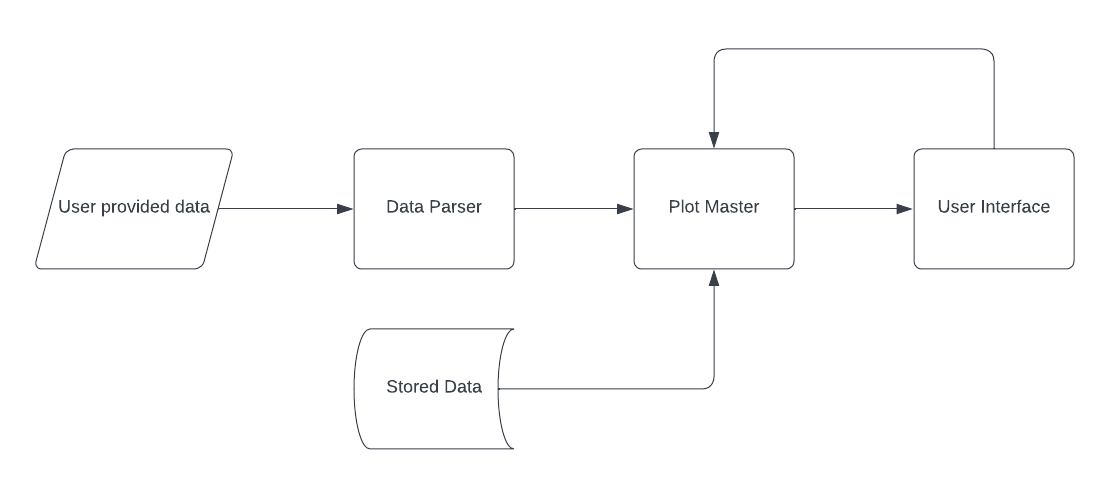
\includegraphics[width=0.9\textwidth]{Figures/Flowchartex1.png}
    \caption{Flowchart}
    \label{fig:flowchart}
\end{figure}

\subsection{Data Parsing}
\label{sec:data-parsing}
A custom parsing solution was developed to read and translate input data necessary for dendrogram visualization. The input data is expected to be put in the "user\textunderscore data" folder. Three files are expected:
\begin{itemize}
    \item heights.csv
    
    Heights refer to the height attribute used in dendrograms. The height attribute represents the heights of individual nodes in the dendrogram in the form of a numeric vector. Each element of the vector is tied to a specific node. Each of the elements measures height from the beginning. 
    
    \item merge.csv

    Merge is a 2D matrix that describes the hierarchical clustering solution. Each row is a description of two components used in a merger. Positive values indicate individual observations (leaf nodes) and negative values indicate clusters formed in previous mergers. More on the iterative process of hierarchical clustering can be read in \ref{sec:hierarchicalclustering}.
    
    \item order.csv

    Order is a vector of positive integers that describes the order in which observations were merged together. The indexing of the data in order.csv is expected to start at 1, as DataParser subtracts 1 from each element to match Python's indexing, which starts at 0. Order is useful for data visualization as it helps the program navigate the easiest way to plot leaves without creating unnecessary cross-overs. 
\end{itemize}

It is also possible to add a fourth file:
\begin{itemize}
    \item labels.csv
    
    Labels is an optional file that should contain a 1D matrix of strings describing each of the datapoints. However, in case the user does not have labels available, mock labels will be provided assigning each element a value from 0 to len(data). 
\end{itemize}

The file format was inspired by the output of R's hclust function.

One file that is not used in plotting the dendrogram is:
\begin{itemize}
    \item data.csv
    
    The data.csv should contain a matrix in which columns represent features and rows represent each of the samples. It can either be raw or preprocessed data. This file is used to plot data represented in dendrogram with the aim to make data exploration more accessible.
\end{itemize}

\subsection{Data Plotting}
\label{sec:data-plotting}
The main component responsible for plotting the data is PlotMaster. The PlotMaster expects data which has been preprocessed by the DataParser. This architecture was selected for merits of having each of the processes split, making it easy to build prototypes in multiple front-end solutions. A well ordered application reduced confusion should the user need to understand anything from the code. 

The PlotMaster leverages Plotly (for deeper description of Plotly see \ref{sec:plotly}) graphing library under the hood. It is designed to help the user explore the data in a visual way. The ability to pan, zoom in, zoom out, or save the plot as .png file is integrated into Plotly. 

There are four types of plots offered by the PlotMaster:
\begin{itemize}
    \item Dendrogram

    Dendrogram is a tree representation of hierarchical clustering as described in \ref{sec:hierarchicalclustering}. The user can interact with the dendrogram by setting color threshold. Color threshold is an integer which is responsible for the height in which clusters are set to different colors, helping the user detect them visually. 
    \begin{figure}[h!]
        \centering
        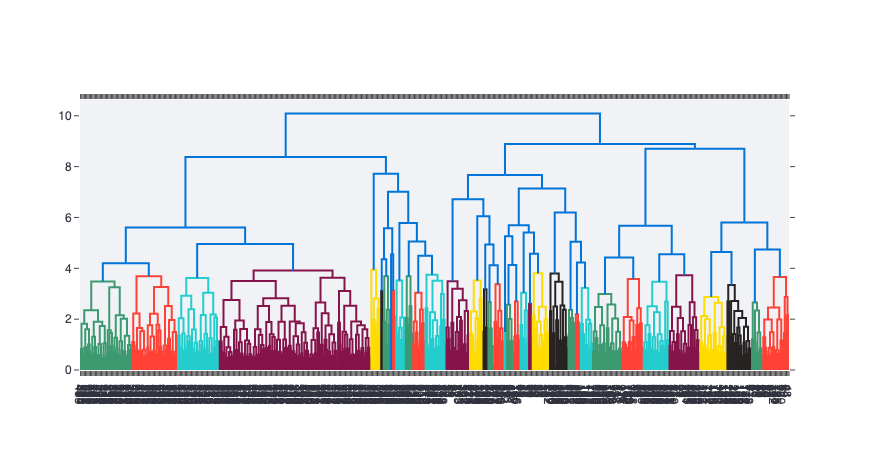
\includegraphics[width=0.9\textwidth]{Figures/dendrogramex.png}
        \caption{Dendrogram}
        \label{fig:dendrogram}
    \end{figure}

    \item Heatmap

    Heatmap is a way to visualize data quantity in color dependent manner as described in \ref{sec:hierarchicalclustering}. The user can specify which features they would like to plot in the available heatmap. 
    \begin{figure}[h!]
        \centering
        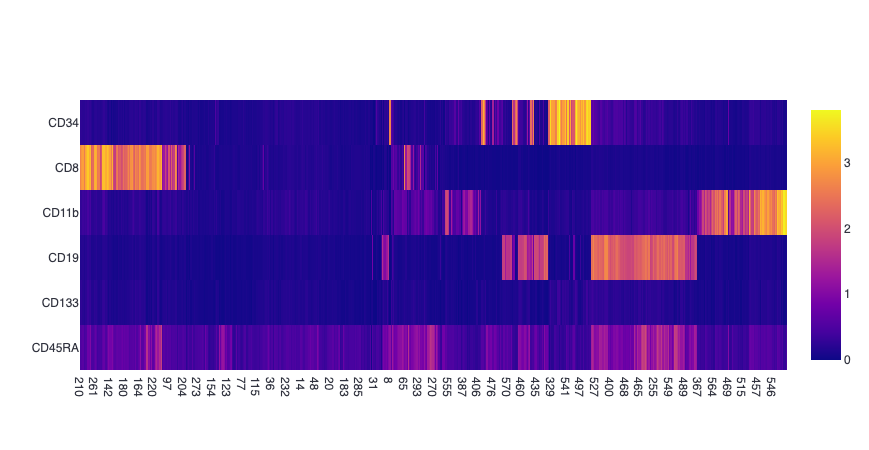
\includegraphics[width=0.9\textwidth]{Figures/heatmapex.png}
        \caption{Heatmap}
        \label{fig:heatmap}
    \end{figure}

    \item 2D exploration of data
    
    The 2D exploration of data offers several options: the selection of two features, scatterplot matrix for all features, and various dimensionality reduction algorithms (PCA, t-SNE, UMAP). The color of each of the datapoints matches the color in the dendrogram. Scatterplot matrix for all features is not recommended for large datasets. 
    
    The PlotMaster searches for data reduction data in the "user\textunderscore data" folder. Should the data not be found it is created by leveraging the sklearn library, and saved in the "user\textunderscore data" folder for later use. 
    
    \begin{figure}[h!]
        \centering
        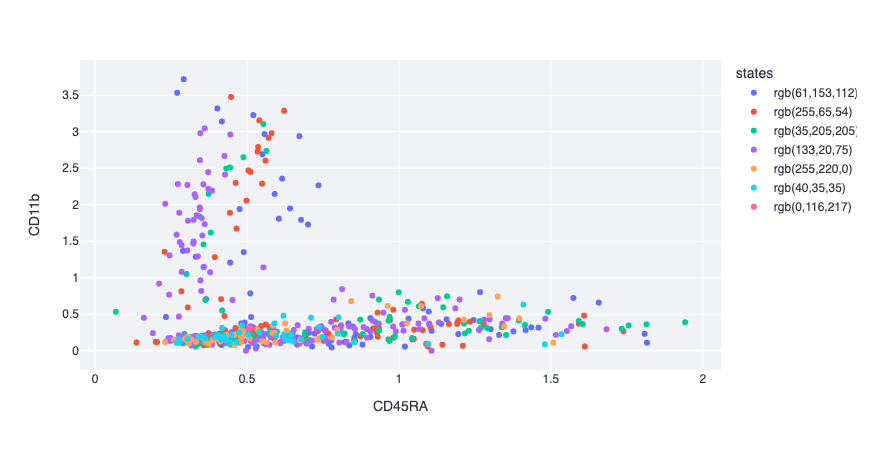
\includegraphics[width=0.9\textwidth]{Figures/twofeat.png}
        \caption{Two Selected Features}
        \label{fig:twofeat}
    \end{figure}

    \item 3D exploration of data
    
    The 3D exploration of data focuses on three dimensionality reduction algorithms: PCA, t-SNE, UMAP. The color of each of the datapoints matches the color in the dendrogram. The user can rotate the plot at will.
    
    The PlotMaster searches for data reduction data in the "user\textunderscore data" folder. Should the data not be found it is created by leveraging the sklearn library, and saved in the "user\textunderscore data" folder for later use. 
    \begin{figure}[h!]
        \centering
        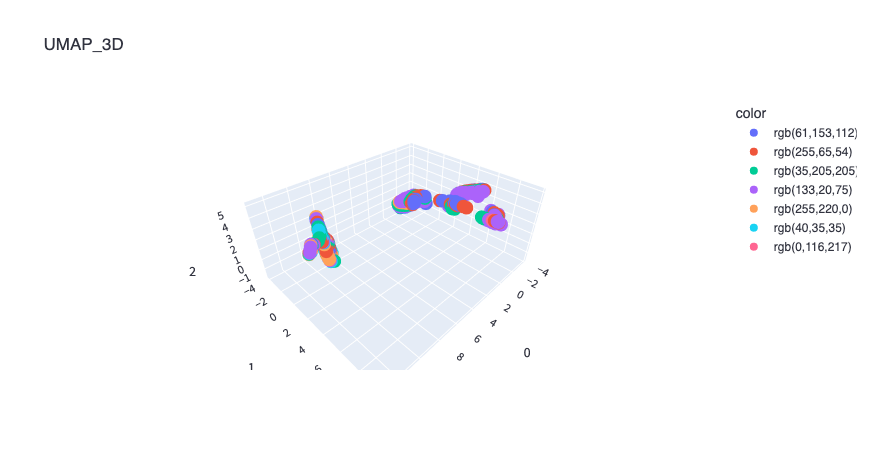
\includegraphics[width=0.9\textwidth]{Figures/umap3d.png}
        \caption{UMAP 3D}
        \label{fig:umap3d}
    \end{figure}
    
\end{itemize}

\newpage
\subsection{User Interface}
\label{sec:userinter}
\paragraph{Streamlit}
\label{sec:st2}
The interface in Streamlit was designed to be simple. Streamlit comes with some formatting out of the box, therefore it is easy to plug it in and have a decent looking application immediately. It also has naive support for Plotly, making it easy to connect the interface to the plotting part of the application. 

For layout, the page configuration was set to wide to make most of users screen's real estate, with two columns. The layout scales with Brave and Chrome browser zoom tool.

On the left, there is a slider, a dropdown menu, and two graph: a dendrogram and a heatmap. The slider is connected to the dendrogram's color threshold, and the user can select any integer from 0 to the maximum value in heights.csv. The dropdown menu allows for selection of multiple values. The values are strings representing features in the dataset. Selected options are plotted in a heatmap, which can be found just under the dendrogram. 

On the right, there is a dropdown menu which allows for selection of multiple options. The offered options are tied to 2D and 3D plots described in \ref{sec:data-plotting}. Plots are displayed in selected order. 

    \begin{figure}[h!]
        \centering
        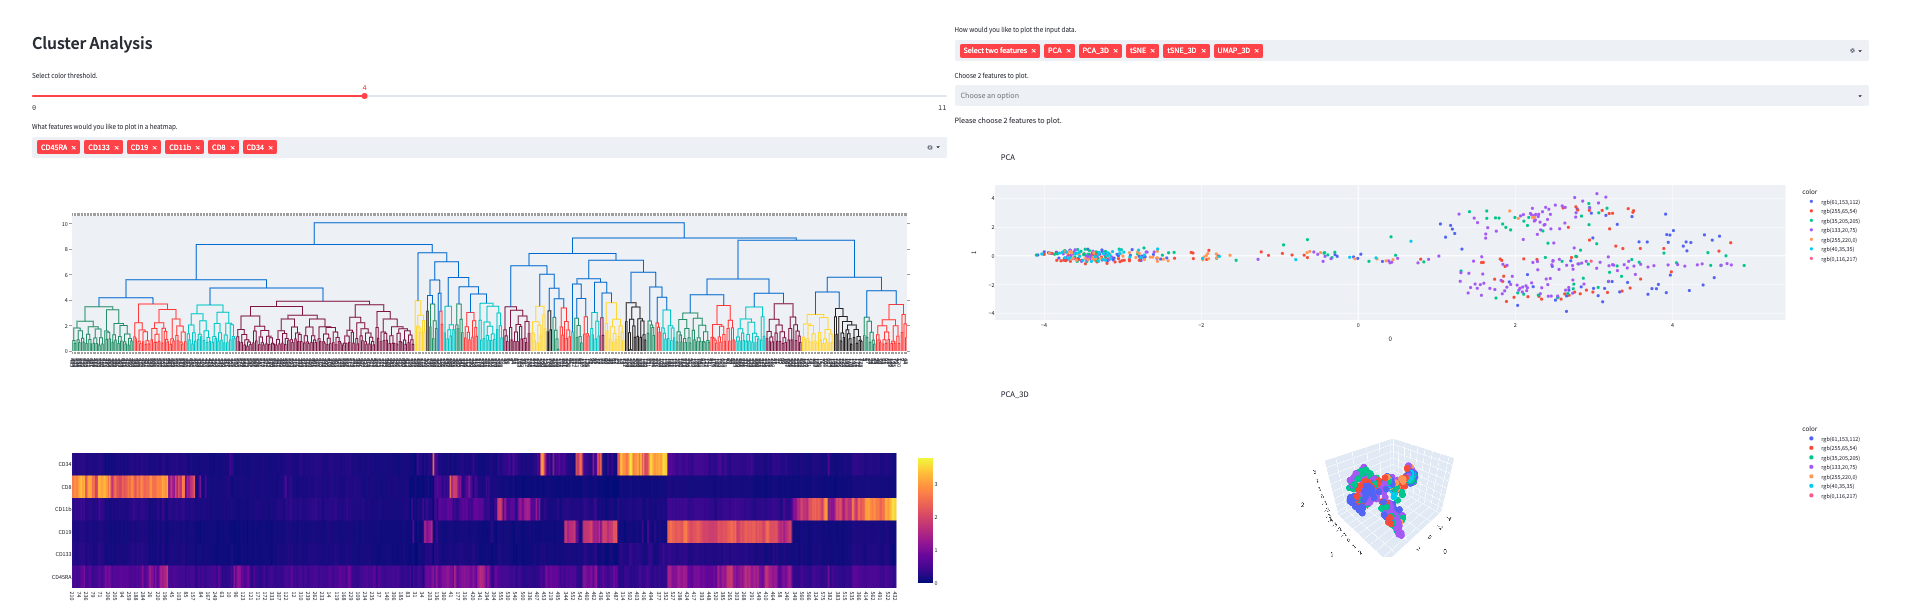
\includegraphics[width=0.9\textwidth]{Figures/streamlit_screen.png}
        \caption{Streamlit Layout}
        \label{fig:streamlay}
    \end{figure}


\newpage
\section{Architecture Challenges}
\label{sec:arch_chal}
\paragraph{Plotly}
\label{sec:plotlych}
Even though Plotly presents itself as a plotting library, it takes care of more than just plotting data. For example, plotly offers a function called create\textunderscore dendrogram, which offers nice tools for working with dendrograms, such as assigning colors, giving reports about each of the leaves, and more. However, the function expects input in the format of raw data, which is incompatible with the input as required from the user (described in \ref{sec:data-parsing}). 

To work around the issue, the function was monkey patched. Monkey patching allows to modify or extend behavior at runtime, eliminating the need to alter the original source code. Thanks to monkey patching the function and underlying Dendrogram class, it was possible to plot the dendrogram data that were obtained from a different algorithm than the one hiding under create\textunderscore dendrogram. 

\paragraph{Streamlit}
\label{sec:st3}
One of the main challenges when working with Streamlit (\ref{sec:streamlit}) is the lack of intelligent interaction with the interactive components provided by the solution. Any time a change is made anywhere, the whole code is rerun, prolonging waiting times for the user. That is also true for components that were not affected by the change. 

Streamlit offers a couple of solutions to the issue. It is recommended to precompute and everything possible, and load the precomputed files into Streamlit instead. 

Another option is to leverage Streamlit's naive cache. The cash promises improved manipulation with large datasets and performing expensive operations. It can be implemented by using the @streamlit.cache decorator on expensive functions. When a function is called with @streamlit.cache decorator, Streamlit checks whether the input parameter has changed, whether any value of any external variable has changed, what is inside the body of the function, and the body of any function called inside the decorated function. Everything is cached the first time the program is run, making the first run more expensive than subsequential runs. 

\paragraph{Dash}
\label{sec:dash3}
A comparable solution was built in Dash, relying on the same PlotMaster background. The lack of out of box formatting was noticable, making the app less pleasant to work with. 

Another challenge was to create a way to share information between each part of the application, since unlike Streamlit, Dash works in a series of callbacks as described in \ref{sec:dash}. Fortunately, Dash offers a data storage components, which enables the communication. 

One of the issues Streamlit brings is that it reruns the whole code whenever anything is changed. It also recomputes all elements that were not subject to the change, making it desirable to implement intermittent data saving and loading to reduce any necessary computation. Streamlit's own caching solution is in development at time of writing this. 

The author found Streamlit's interface easier to navigate by a small margin, and integrated formatting out the box makes the application look more well rounded compared to out of the box bareness of Dash, which expects user specified formatting, ideally in the form of a .css file.

\chapter{Results} 
\label{chap:seven}
XXX
  










\chapter{Concluding Remarks}
\label{chap:eight}

XXX


\clearpage
%-----<<< -------- >>>-----

%-----<<< REFERENCES >>>-----
\fancyhead[LO]{\sffamily Bibliography}					%headers in sans serif and not in uppercase
\bibliographystyle{Styles/Stylebib}							%style of literature, you can use e.g. newapa	instead of Styles/Stylebib
\bibliography{Styles/Bibliography}							%bibliography database
\addcontentsline{toc}{chapter}{Bibliography} 		%Add bibliography to the table of contents
\clearpage
%-----<<< ---------- >>>-----

%-----<<< APPENDIXES >>>-----
\backmatter																			%uppercase roman pagination for back matter; appendices start
\autohdr																				%automatic headers     				
\chapter{Appendix One}

\section{Derivation of Desired Sample Size}
\label{Apendix:Hoef}
XXX

           			%input file
\chapter{R Source Codes}
\section{R Source Code for Dataset and Result Generation}
\begin{lstlisting}[breaklines]
XXX

\end{lstlisting}
           			%input file
\clearpage
%-----<<< --------- >>>-----

\end{document}
%-----<<<<<<<<< END OF DOCUMENT >>>>>>>>>-----
